% Options for packages loaded elsewhere
\PassOptionsToPackage{unicode}{hyperref}
\PassOptionsToPackage{hyphens}{url}
%
\documentclass[
]{article}
\usepackage{amsmath,amssymb}
\usepackage{lmodern}
\usepackage{iftex}
\ifPDFTeX
  \usepackage[T1]{fontenc}
  \usepackage[utf8]{inputenc}
  \usepackage{textcomp} % provide euro and other symbols
\else % if luatex or xetex
  \usepackage{unicode-math}
  \defaultfontfeatures{Scale=MatchLowercase}
  \defaultfontfeatures[\rmfamily]{Ligatures=TeX,Scale=1}
\fi
% Use upquote if available, for straight quotes in verbatim environments
\IfFileExists{upquote.sty}{\usepackage{upquote}}{}
\IfFileExists{microtype.sty}{% use microtype if available
  \usepackage[]{microtype}
  \UseMicrotypeSet[protrusion]{basicmath} % disable protrusion for tt fonts
}{}
\makeatletter
\@ifundefined{KOMAClassName}{% if non-KOMA class
  \IfFileExists{parskip.sty}{%
    \usepackage{parskip}
  }{% else
    \setlength{\parindent}{0pt}
    \setlength{\parskip}{6pt plus 2pt minus 1pt}}
}{% if KOMA class
  \KOMAoptions{parskip=half}}
\makeatother
\usepackage{xcolor}
\usepackage[margin=1in]{geometry}
\usepackage{color}
\usepackage{fancyvrb}
\newcommand{\VerbBar}{|}
\newcommand{\VERB}{\Verb[commandchars=\\\{\}]}
\DefineVerbatimEnvironment{Highlighting}{Verbatim}{commandchars=\\\{\}}
% Add ',fontsize=\small' for more characters per line
\newenvironment{Shaded}{}{}
\newcommand{\AlertTok}[1]{\textbf{#1}}
\newcommand{\AnnotationTok}[1]{\textit{#1}}
\newcommand{\AttributeTok}[1]{#1}
\newcommand{\BaseNTok}[1]{#1}
\newcommand{\BuiltInTok}[1]{#1}
\newcommand{\CharTok}[1]{#1}
\newcommand{\CommentTok}[1]{\textit{#1}}
\newcommand{\CommentVarTok}[1]{\textit{#1}}
\newcommand{\ConstantTok}[1]{#1}
\newcommand{\ControlFlowTok}[1]{\textbf{#1}}
\newcommand{\DataTypeTok}[1]{\underline{#1}}
\newcommand{\DecValTok}[1]{#1}
\newcommand{\DocumentationTok}[1]{\textit{#1}}
\newcommand{\ErrorTok}[1]{\textbf{#1}}
\newcommand{\ExtensionTok}[1]{#1}
\newcommand{\FloatTok}[1]{#1}
\newcommand{\FunctionTok}[1]{#1}
\newcommand{\ImportTok}[1]{#1}
\newcommand{\InformationTok}[1]{\textit{#1}}
\newcommand{\KeywordTok}[1]{\textbf{#1}}
\newcommand{\NormalTok}[1]{#1}
\newcommand{\OperatorTok}[1]{#1}
\newcommand{\OtherTok}[1]{#1}
\newcommand{\PreprocessorTok}[1]{\textbf{#1}}
\newcommand{\RegionMarkerTok}[1]{#1}
\newcommand{\SpecialCharTok}[1]{#1}
\newcommand{\SpecialStringTok}[1]{#1}
\newcommand{\StringTok}[1]{#1}
\newcommand{\VariableTok}[1]{#1}
\newcommand{\VerbatimStringTok}[1]{#1}
\newcommand{\WarningTok}[1]{\textit{#1}}
\usepackage{longtable,booktabs,array}
\usepackage{calc} % for calculating minipage widths
% Correct order of tables after \paragraph or \subparagraph
\usepackage{etoolbox}
\makeatletter
\patchcmd\longtable{\par}{\if@noskipsec\mbox{}\fi\par}{}{}
\makeatother
% Allow footnotes in longtable head/foot
\IfFileExists{footnotehyper.sty}{\usepackage{footnotehyper}}{\usepackage{footnote}}
\makesavenoteenv{longtable}
\usepackage{graphicx}
\makeatletter
\def\maxwidth{\ifdim\Gin@nat@width>\linewidth\linewidth\else\Gin@nat@width\fi}
\def\maxheight{\ifdim\Gin@nat@height>\textheight\textheight\else\Gin@nat@height\fi}
\makeatother
% Scale images if necessary, so that they will not overflow the page
% margins by default, and it is still possible to overwrite the defaults
% using explicit options in \includegraphics[width, height, ...]{}
\setkeys{Gin}{width=\maxwidth,height=\maxheight,keepaspectratio}
% Set default figure placement to htbp
\makeatletter
\def\fps@figure{htbp}
\makeatother
\setlength{\emergencystretch}{3em} % prevent overfull lines
\providecommand{\tightlist}{%
  \setlength{\itemsep}{0pt}\setlength{\parskip}{0pt}}
\setcounter{secnumdepth}{5}
\usepackage{float} \floatplacement{figure}{H} \usepackage{fvextra} \DefineVerbatimEnvironment{Highlighting}{Verbatim}{breaklines,commandchars=\\\{\}} \usepackage[format=plain,labelfont={bf,it},textfont={}]{caption} \usepackage{booktabs} \usepackage{longtable} \usepackage{lscape} \newcommand{\blandscape}{\begin{landscape}} \newcommand{\elandscape}{\end{landscape}}
\usepackage{booktabs}
\usepackage{longtable}
\usepackage{array}
\usepackage{multirow}
\usepackage{wrapfig}
\usepackage{float}
\usepackage{colortbl}
\usepackage{pdflscape}
\usepackage{tabu}
\usepackage{threeparttable}
\usepackage{threeparttablex}
\usepackage[normalem]{ulem}
\usepackage{makecell}
\usepackage{xcolor}
\ifLuaTeX
  \usepackage{selnolig}  % disable illegal ligatures
\fi
\IfFileExists{bookmark.sty}{\usepackage{bookmark}}{\usepackage{hyperref}}
\IfFileExists{xurl.sty}{\usepackage{xurl}}{} % add URL line breaks if available
\urlstyle{same} % disable monospaced font for URLs
\hypersetup{
  pdftitle={Pharmacogenomics Next Generation Sequencing Run Quality Control Metrics},
  pdfauthor={Galenvs Sciences Inc.},
  hidelinks,
  pdfcreator={LaTeX via pandoc}}

\title{Pharmacogenomics Next Generation Sequencing Run Quality Control Metrics}
\author{Galenvs Sciences Inc.}
\date{14 July, 2023}

\begin{document}
\maketitle

\hypertarget{summary}{%
\section{Summary}\label{summary}}

\begin{longtable}[t]{>{\raggedright\arraybackslash}p{2cm}>{\raggedright\arraybackslash}p{2cm}>{\raggedright\arraybackslash}p{1.6cm}>{\raggedright\arraybackslash}p{3cm}>{\raggedright\arraybackslash}p{1.6cm}>{}l}
\caption{(\#tab:unnamed-chunk-1)Summary of QC check results.}\\
\toprule
Barcode ID & Sample Name & Depth QC Check & Uniformity QC Check & Coverage QC Check & Overall QC Checkpoint\\
\midrule
IonCode\_0121 & Sample 1 & PASS & ACCEPTABLE & PASS & \textcolor{olive}{PASS}\\
IonCode\_0122 & Sample 2 & PASS & ACCEPTABLE & PASS & \textcolor{olive}{PASS}\\
IonCode\_0123 & Sample 3 & PASS & FAIL & PASS & \textcolor{red}{FAIL}\\
IonCode\_0124 & Sample 4 & PASS & ACCEPTABLE & PASS & \textcolor{olive}{PASS}\\
IonCode\_0125 & Sample 5 & PASS & ACCEPTABLE & PASS & \textcolor{olive}{PASS}\\
\addlinespace
IonCode\_0126 & Sample 6 & PASS & ACCEPTABLE & PASS & \textcolor{olive}{PASS}\\
IonCode\_0127 & Sample 7 & PASS & ACCEPTABLE & PASS & \textcolor{olive}{PASS}\\
IonCode\_0128 & Sample 8 & PASS & FAIL & PASS & \textcolor{red}{FAIL}\\
IonCode\_0129 & Sample 9 & PASS & ACCEPTABLE & PASS & \textcolor{olive}{PASS}\\
IonCode\_0130 & Sample 10 & PASS & FAIL & PASS & \textcolor{red}{FAIL}\\
\addlinespace
IonCode\_0131 & Sample 11 & PASS & FAIL & FAIL & \textcolor{red}{FAIL}\\
IonCode\_0132 & Sample 12 & PASS & ACCEPTABLE & PASS & \textcolor{olive}{PASS}\\
IonCode\_0133 & Sample 13 & PASS & ACCEPTABLE & PASS & \textcolor{olive}{PASS}\\
IonCode\_0134 & Sample 14 & PASS & ACCEPTABLE & PASS & \textcolor{olive}{PASS}\\
\bottomrule
\end{longtable}
\newpage

\tableofcontents

\newpage

\hypertarget{base-depth}{%
\section{Base Depth}\label{base-depth}}

\hypertarget{mean-depth}{%
\subsection{Mean Depth}\label{mean-depth}}

The mean depth for each sample is shown in \textbf{\emph{table @ref(tab:meanDepthResults)}}.

\begin{longtable}[t]{llrl}
\caption{(\#tab:meanDepthResults)Mean Depth Results.}\\
\toprule
Barcode ID & Sample Name & Mean Depth & Depth QC Check\\
\midrule
IonCode\_0121 & Sample 1 & 10763 & PASS\\
IonCode\_0122 & Sample 2 & 13867 & PASS\\
IonCode\_0123 & Sample 3 & 9712 & PASS\\
IonCode\_0124 & Sample 4 & 6887 & PASS\\
IonCode\_0125 & Sample 5 & 7129 & PASS\\
\addlinespace
IonCode\_0126 & Sample 6 & 7081 & PASS\\
IonCode\_0127 & Sample 7 & 8287 & PASS\\
IonCode\_0128 & Sample 8 & 11103 & PASS\\
IonCode\_0129 & Sample 9 & 7582 & PASS\\
IonCode\_0130 & Sample 10 & 8432 & PASS\\
\addlinespace
IonCode\_0131 & Sample 11 & 8082 & PASS\\
IonCode\_0132 & Sample 12 & 8402 & PASS\\
IonCode\_0133 & Sample 13 & 6474 & PASS\\
IonCode\_0134 & Sample 14 & 7504 & PASS\\
\bottomrule
\end{longtable}

\hypertarget{regions-with-100-bases-read-500x-by-sample}{%
\subsection{Regions with \textless100\% Bases Read 500X (by Sample)}\label{regions-with-100-bases-read-500x-by-sample}}

The distribution of the fraction of bases read 500X in a given amplicon is shown in \textbf{\emph{figure @ref(fig:depthHeatmap)}}.

\begin{figure}
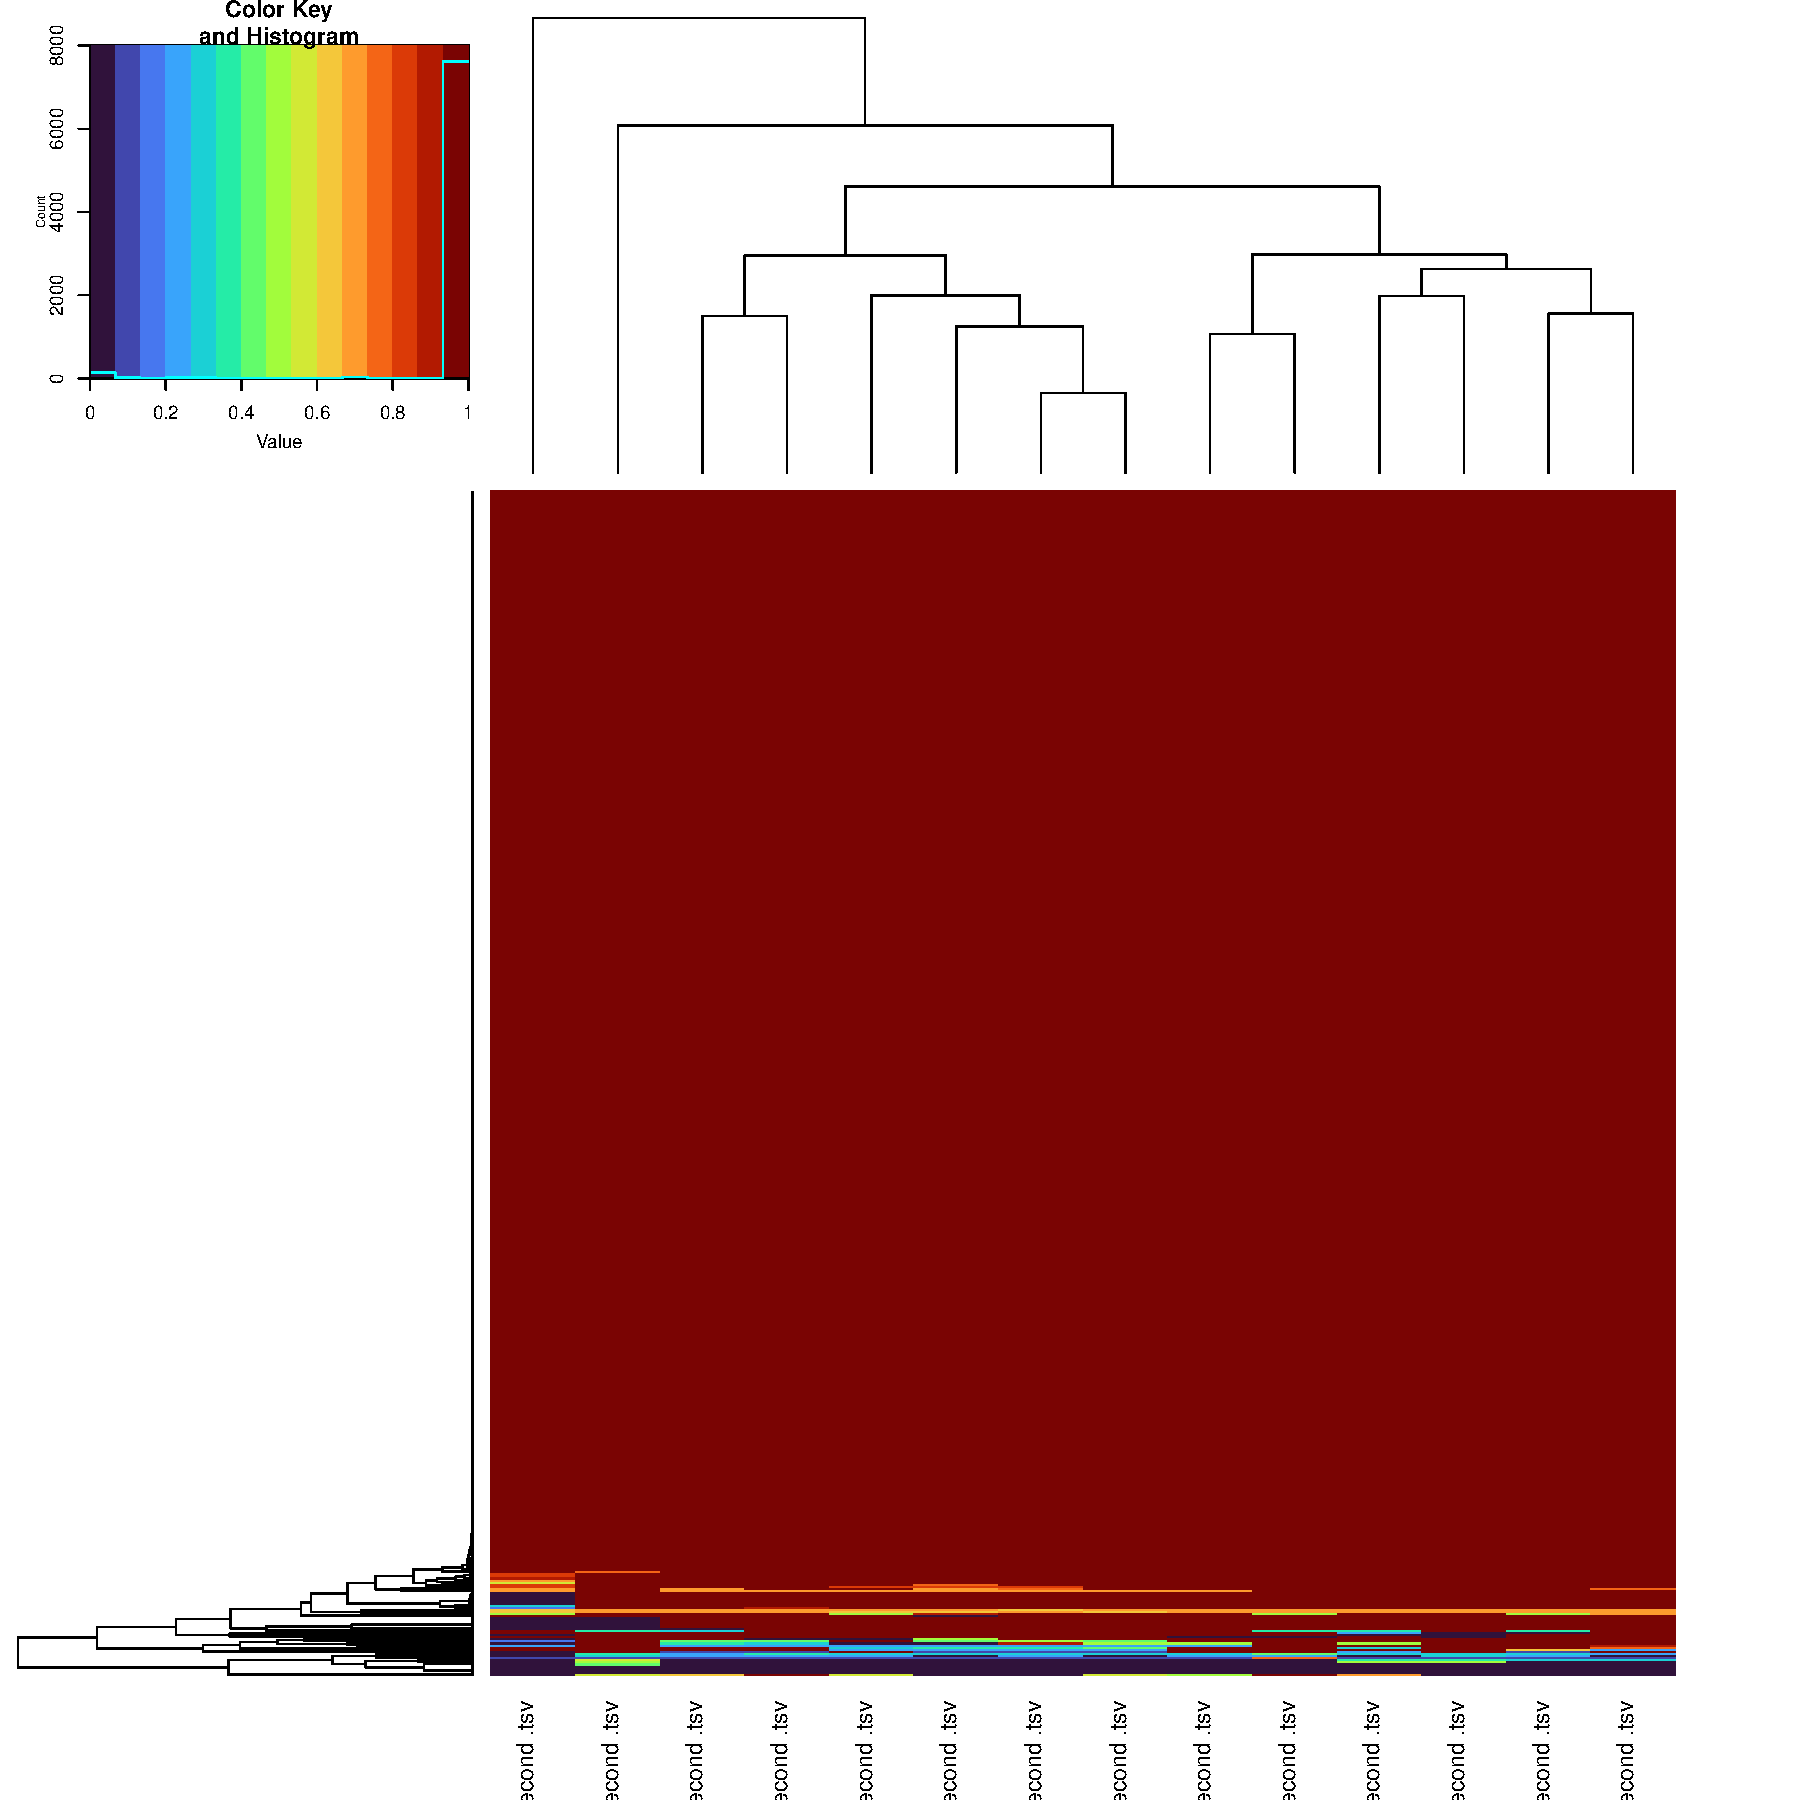
\includegraphics{C:\Users\jonat\Desktop\ngs_app_galenvs\server\records\experiment_data_140723_1449_the one\report_files/figure-latex/depthHeatmap-1} \caption[Depth 500X Heatmap]{Heatmap showing the distribution of the fraction of bases read 500X in a given amplicon. Rows represent amplicons and columns represent samples}(\#fig:depthHeatmap)
\end{figure}

The following regions do not meet the criteria of having 100\% of bases read 500X (by sample). The total number of unique regions that do not meet this criteria across samples is 69 regions.

\begin{Shaded}
\begin{Highlighting}[]
\NormalTok{\#\# $\textasciigrave{}experiment\_data\_140723\_1108\_day second /depth\_140723\_1108\_day second /depth\_01\_140723\_1108\_day second .tsv\textasciigrave{}}
\NormalTok{\#\# $\textasciigrave{}experiment\_data\_140723\_1108\_day second /depth\_140723\_1108\_day second /depth\_01\_140723\_1108\_day second .tsv\textasciigrave{}$region\_id}
\NormalTok{\#\#  [1] "AMPL3925991" "AMPL3926426" "AMPL3926093" "AMPL3926201" "AMPL3926248"}
\NormalTok{\#\#  [6] "AMPL3926466" "AMPL3926510" "AMPL2649381" "AMPL3925990" "AMPL3926044"}
\NormalTok{\#\# [11] "AMPL3926172" "AMPL3091682" "AMPL3926529" "AMPL3926313" "AMPL3926668"}
\NormalTok{\#\# [16] "AMPL3926182" "AMPL3926491" "AMPL3925971" "AMPL3926501" "AMPL3926165"}
\NormalTok{\#\# [21] "AMPL3926019" "AMPL2654393" "AMPL2686855"}
\NormalTok{\#\# }
\NormalTok{\#\# }
\NormalTok{\#\# $\textasciigrave{}experiment\_data\_140723\_1108\_day second /depth\_140723\_1108\_day second /depth\_02\_140723\_1108\_day second .tsv\textasciigrave{}}
\NormalTok{\#\# $\textasciigrave{}experiment\_data\_140723\_1108\_day second /depth\_140723\_1108\_day second /depth\_02\_140723\_1108\_day second .tsv\textasciigrave{}$region\_id}
\NormalTok{\#\#  [1] "AMPL3925991" "AMPL3926277" "AMPL3925943" "AMPL3926515" "AMPL3926625"}
\NormalTok{\#\#  [6] "AMPL3926052" "AMPL3926072" "AMPL3926201" "AMPL3926093" "AMPL3926510"}
\NormalTok{\#\# [11] "AMPL3926426" "AMPL3926248" "AMPL2649381" "AMPL3925990" "AMPL3091682"}
\NormalTok{\#\# [16] "AMPL3926313" "AMPL3926095" "AMPL3926172" "AMPL3926466" "AMPL3926166"}
\NormalTok{\#\# [21] "AMPL3926668" "AMPL3926491" "AMPL3925971" "AMPL3926036" "AMPL3926019"}
\NormalTok{\#\# [26] "AMPL3926448" "AMPL2654393"}
\NormalTok{\#\# }
\NormalTok{\#\# }
\NormalTok{\#\# $\textasciigrave{}experiment\_data\_140723\_1108\_day second /depth\_140723\_1108\_day second /depth\_03\_140723\_1108\_day second .tsv\textasciigrave{}}
\NormalTok{\#\# $\textasciigrave{}experiment\_data\_140723\_1108\_day second /depth\_140723\_1108\_day second /depth\_03\_140723\_1108\_day second .tsv\textasciigrave{}$region\_id}
\NormalTok{\#\#  [1] "AMPL3926668" "AMPL3925991" "AMPL3926093" "AMPL3697894" "AMPL3926201"}
\NormalTok{\#\#  [6] "AMPL3926510" "AMPL3926426" "AMPL3925990" "AMPL3925968" "AMPL3926313"}
\NormalTok{\#\# [11] "AMPL3926248" "AMPL3926172" "AMPL2649381" "AMPL3922006" "AMPL3926095"}
\NormalTok{\#\# [16] "AMPL3091682" "AMPL3926466" "AMPL3926295" "AMPL3926491" "AMPL3926165"}
\NormalTok{\#\# [21] "AMPL3925971" "AMPL3926546" "AMPL3926019" "AMPL3926204" "AMPL3926556"}
\NormalTok{\#\# [26] "AMPL3926448" "AMPL2654393"}
\NormalTok{\#\# }
\NormalTok{\#\# }
\NormalTok{\#\# $\textasciigrave{}experiment\_data\_140723\_1108\_day second /depth\_140723\_1108\_day second /depth\_04\_140723\_1108\_day second .tsv\textasciigrave{}}
\NormalTok{\#\# $\textasciigrave{}experiment\_data\_140723\_1108\_day second /depth\_140723\_1108\_day second /depth\_04\_140723\_1108\_day second .tsv\textasciigrave{}$region\_id}
\NormalTok{\#\#  [1] "AMPL3925991" "AMPL3926093" "AMPL3926201" "AMPL3926313" "AMPL3926466"}
\NormalTok{\#\#  [6] "AMPL3926510" "AMPL3926426" "AMPL3925990" "AMPL2649381" "AMPL3091682"}
\NormalTok{\#\# [11] "AMPL3926248" "AMPL3926476" "AMPL3926044" "AMPL3925912" "AMPL3926668"}
\NormalTok{\#\# [16] "AMPL3926172" "AMPL3925971" "AMPL3926491" "AMPL3926247" "AMPL3926573"}
\NormalTok{\#\# [21] "AMPL3926367" "AMPL3926165" "AMPL3926019" "AMPL3926339" "AMPL3925922"}
\NormalTok{\#\# [26] "AMPL3926501" "AMPL2686855" "AMPL2654393"}
\NormalTok{\#\# }
\NormalTok{\#\# }
\NormalTok{\#\# $\textasciigrave{}experiment\_data\_140723\_1108\_day second /depth\_140723\_1108\_day second /depth\_05\_140723\_1108\_day second .tsv\textasciigrave{}}
\NormalTok{\#\# $\textasciigrave{}experiment\_data\_140723\_1108\_day second /depth\_140723\_1108\_day second /depth\_05\_140723\_1108\_day second .tsv\textasciigrave{}$region\_id}
\NormalTok{\#\#  [1] "AMPL3925991" "AMPL3926668" "AMPL3926093" "AMPL3926201" "AMPL3926466"}
\NormalTok{\#\#  [6] "AMPL3926426" "AMPL3926510" "AMPL2649381" "AMPL3926248" "AMPL3091682"}
\NormalTok{\#\# [11] "AMPL3925990" "AMPL3698522" "AMPL3926517" "AMPL3926172" "AMPL3925912"}
\NormalTok{\#\# [16] "AMPL3926313" "AMPL3926491" "AMPL3925971" "AMPL3926386" "AMPL3926501"}
\NormalTok{\#\# [21] "AMPL3926165" "AMPL3926019" "AMPL2683406" "AMPL3926155" "AMPL3926002"}
\NormalTok{\#\# [26] "AMPL3926367" "AMPL3926339" "AMPL3925922" "AMPL2654393" "AMPL2686855"}
\NormalTok{\#\# [31] "AMPL3926591"}
\NormalTok{\#\# }
\NormalTok{\#\# }
\NormalTok{\#\# $\textasciigrave{}experiment\_data\_140723\_1108\_day second /depth\_140723\_1108\_day second /depth\_06\_140723\_1108\_day second .tsv\textasciigrave{}}
\NormalTok{\#\# $\textasciigrave{}experiment\_data\_140723\_1108\_day second /depth\_140723\_1108\_day second /depth\_06\_140723\_1108\_day second .tsv\textasciigrave{}$region\_id}
\NormalTok{\#\#  [1] "AMPL3926668" "AMPL3925991" "AMPL3926093" "AMPL3926201" "AMPL3926466"}
\NormalTok{\#\#  [6] "AMPL3926426" "AMPL3926248" "AMPL3926510" "AMPL3091682" "AMPL3926313"}
\NormalTok{\#\# [11] "AMPL3925990" "AMPL3926172" "AMPL2649381" "AMPL3926517" "AMPL3926044"}
\NormalTok{\#\# [16] "AMPL3926386" "AMPL3925971" "AMPL3926501" "AMPL3926491" "AMPL3926165"}
\NormalTok{\#\# [21] "AMPL3926367" "AMPL2683406" "AMPL3926019" "AMPL3925922" "AMPL3926339"}
\NormalTok{\#\# [26] "AMPL2654393" "AMPL2686855" "AMPL3926591"}
\NormalTok{\#\# }
\NormalTok{\#\# }
\NormalTok{\#\# $\textasciigrave{}experiment\_data\_140723\_1108\_day second /depth\_140723\_1108\_day second /depth\_07\_140723\_1108\_day second .tsv\textasciigrave{}}
\NormalTok{\#\# $\textasciigrave{}experiment\_data\_140723\_1108\_day second /depth\_140723\_1108\_day second /depth\_07\_140723\_1108\_day second .tsv\textasciigrave{}$region\_id}
\NormalTok{\#\#  [1] "AMPL3926668" "AMPL3925991" "AMPL3926093" "AMPL3926201" "AMPL3926510"}
\NormalTok{\#\#  [6] "AMPL3926426" "AMPL3925990" "AMPL3091682" "AMPL3926313" "AMPL2649381"}
\NormalTok{\#\# [11] "AMPL3926466" "AMPL3926172" "AMPL3926491" "AMPL3925971" "AMPL3926165"}
\NormalTok{\#\# [16] "AMPL3926155" "AMPL2683406" "AMPL3926367" "AMPL3926019" "AMPL3926339"}
\NormalTok{\#\# [21] "AMPL2686855" "AMPL2654393"}
\NormalTok{\#\# }
\NormalTok{\#\# }
\NormalTok{\#\# $\textasciigrave{}experiment\_data\_140723\_1108\_day second /depth\_140723\_1108\_day second /depth\_08\_140723\_1108\_day second .tsv\textasciigrave{}}
\NormalTok{\#\# $\textasciigrave{}experiment\_data\_140723\_1108\_day second /depth\_140723\_1108\_day second /depth\_08\_140723\_1108\_day second .tsv\textasciigrave{}$region\_id}
\NormalTok{\#\#  [1] "AMPL3926313" "AMPL3925991" "AMPL3926512" "AMPL3697894" "AMPL3926093"}
\NormalTok{\#\#  [6] "AMPL3926201" "AMPL3926426" "AMPL3926510" "AMPL3925968" "AMPL3547871"}
\NormalTok{\#\# [11] "AMPL3925990" "AMPL2649381" "AMPL3091682" "AMPL3926248" "AMPL3926466"}
\NormalTok{\#\# [16] "AMPL3926172" "AMPL3926668" "AMPL3926491" "AMPL3925971" "AMPL2683406"}
\NormalTok{\#\# [21] "AMPL3926165" "AMPL3926019" "AMPL2654393"}
\NormalTok{\#\# }
\NormalTok{\#\# }
\NormalTok{\#\# $\textasciigrave{}experiment\_data\_140723\_1108\_day second /depth\_140723\_1108\_day second /depth\_09\_140723\_1108\_day second .tsv\textasciigrave{}}
\NormalTok{\#\# $\textasciigrave{}experiment\_data\_140723\_1108\_day second /depth\_140723\_1108\_day second /depth\_09\_140723\_1108\_day second .tsv\textasciigrave{}$region\_id}
\NormalTok{\#\#  [1] "AMPL3926512" "AMPL3925991" "AMPL3926201" "AMPL3926510" "AMPL3091682"}
\NormalTok{\#\#  [6] "AMPL3925990" "AMPL2649381" "AMPL3926426" "AMPL3926093" "AMPL3926466"}
\NormalTok{\#\# [11] "AMPL3926248" "AMPL3926668" "AMPL3926172" "AMPL3926095" "AMPL3926313"}
\NormalTok{\#\# [16] "AMPL3925971" "AMPL3926491" "AMPL3926632" "AMPL3926002" "AMPL3926339"}
\NormalTok{\#\# [21] "AMPL3926165" "AMPL3926019" "AMPL3926448" "AMPL2686855" "AMPL2654393"}
\NormalTok{\#\# }
\NormalTok{\#\# }
\NormalTok{\#\# $\textasciigrave{}experiment\_data\_140723\_1108\_day second /depth\_140723\_1108\_day second /depth\_10\_140723\_1108\_day second .tsv\textasciigrave{}}
\NormalTok{\#\# $\textasciigrave{}experiment\_data\_140723\_1108\_day second /depth\_140723\_1108\_day second /depth\_10\_140723\_1108\_day second .tsv\textasciigrave{}$region\_id}
\NormalTok{\#\#  [1] "AMPL3925991" "AMPL3926313" "AMPL3926093" "AMPL3926201" "AMPL3926426"}
\NormalTok{\#\#  [6] "AMPL3926510" "AMPL3926248" "AMPL3925990" "AMPL3925968" "AMPL2649381"}
\NormalTok{\#\# [11] "AMPL3091682" "AMPL3922006" "AMPL3926172" "AMPL3926095" "AMPL3926466"}
\NormalTok{\#\# [16] "AMPL3926386" "AMPL3926668" "AMPL3925914" "AMPL3926491" "AMPL3926339"}
\NormalTok{\#\# [21] "AMPL3926036" "AMPL2683406" "AMPL3925971" "AMPL3926019" "AMPL3926591"}
\NormalTok{\#\# [26] "AMPL3926448" "AMPL2654393"}
\NormalTok{\#\# }
\NormalTok{\#\# }
\NormalTok{\#\# $\textasciigrave{}experiment\_data\_140723\_1108\_day second /depth\_140723\_1108\_day second /depth\_11\_140723\_1108\_day second .tsv\textasciigrave{}}
\NormalTok{\#\# $\textasciigrave{}experiment\_data\_140723\_1108\_day second /depth\_140723\_1108\_day second /depth\_11\_140723\_1108\_day second .tsv\textasciigrave{}$region\_id}
\NormalTok{\#\#  [1] "AMPL3697894" "AMPL3926277" "AMPL3926172" "AMPL3925991" "AMPL3926625"}
\NormalTok{\#\#  [6] "AMPL3926052" "AMPL3925943" "AMPL3926093" "AMPL3926515" "AMPL3926248"}
\NormalTok{\#\# [11] "AMPL3926072" "AMPL3926201" "AMPL3926426" "AMPL3925990" "AMPL2649381"}
\NormalTok{\#\# [16] "AMPL3926044" "AMPL3926529" "AMPL3926313" "AMPL3926466" "AMPL3926088"}
\NormalTok{\#\# [21] "AMPL3926668" "AMPL3091682" "AMPL3926510" "AMPL3698522" "AMPL3926386"}
\NormalTok{\#\# [26] "AMPL3926491" "AMPL3219749" "AMPL3925912" "AMPL3922006" "AMPL3698542"}
\NormalTok{\#\# [31] "AMPL3926349" "AMPL2654412" "AMPL3926354" "AMPL3926579" "AMPL2683245"}
\NormalTok{\#\# [36] "AMPL3926539" "AMPL3926470" "AMPL3925971" "AMPL2683406" "AMPL3926546"}
\NormalTok{\#\# [41] "AMPL3926019" "AMPL3926036" "AMPL3926367" "AMPL3926501" "AMPL3926204"}
\NormalTok{\#\# [46] "AMPL3925922" "AMPL3926591" "AMPL3926556" "AMPL2686855" "AMPL2654393"}
\NormalTok{\#\# }
\NormalTok{\#\# }
\NormalTok{\#\# $\textasciigrave{}experiment\_data\_140723\_1108\_day second /depth\_140723\_1108\_day second /depth\_12\_140723\_1108\_day second .tsv\textasciigrave{}}
\NormalTok{\#\# $\textasciigrave{}experiment\_data\_140723\_1108\_day second /depth\_140723\_1108\_day second /depth\_12\_140723\_1108\_day second .tsv\textasciigrave{}$region\_id}
\NormalTok{\#\#  [1] "AMPL3925991" "AMPL3926625" "AMPL3926426" "AMPL3926201" "AMPL3926248"}
\NormalTok{\#\#  [6] "AMPL3926510" "AMPL3926093" "AMPL3926466" "AMPL2649381" "AMPL3091682"}
\NormalTok{\#\# [11] "AMPL3926095" "AMPL3925990" "AMPL3926313" "AMPL3926172" "AMPL3926668"}
\NormalTok{\#\# [16] "AMPL3926491" "AMPL3925971" "AMPL3926501" "AMPL3926339" "AMPL3926367"}
\NormalTok{\#\# [21] "AMPL3926019" "AMPL3926573" "AMPL3926448" "AMPL2686855" "AMPL2654393"}
\NormalTok{\#\# }
\NormalTok{\#\# }
\NormalTok{\#\# $\textasciigrave{}experiment\_data\_140723\_1108\_day second /depth\_140723\_1108\_day second /depth\_13\_140723\_1108\_day second .tsv\textasciigrave{}}
\NormalTok{\#\# $\textasciigrave{}experiment\_data\_140723\_1108\_day second /depth\_140723\_1108\_day second /depth\_13\_140723\_1108\_day second .tsv\textasciigrave{}$region\_id}
\NormalTok{\#\#  [1] "AMPL3925991" "AMPL3926093" "AMPL3926201" "AMPL3926466" "AMPL3926510"}
\NormalTok{\#\#  [6] "AMPL3926426" "AMPL2649381" "AMPL3091682" "AMPL3926044" "AMPL3925990"}
\NormalTok{\#\# [11] "AMPL3926172" "AMPL3926248" "AMPL3925912" "AMPL3926668" "AMPL3926491"}
\NormalTok{\#\# [16] "AMPL3926313" "AMPL3925971" "AMPL3926165" "AMPL3926002" "AMPL3926367"}
\NormalTok{\#\# [21] "AMPL3926019" "AMPL3925922" "AMPL3926339" "AMPL2686855" "AMPL2654393"}
\NormalTok{\#\# [26] "AMPL3925962"}
\NormalTok{\#\# }
\NormalTok{\#\# }
\NormalTok{\#\# $\textasciigrave{}experiment\_data\_140723\_1108\_day second /depth\_140723\_1108\_day second /depth\_14\_140723\_1108\_day second .tsv\textasciigrave{}}
\NormalTok{\#\# $\textasciigrave{}experiment\_data\_140723\_1108\_day second /depth\_140723\_1108\_day second /depth\_14\_140723\_1108\_day second .tsv\textasciigrave{}$region\_id}
\NormalTok{\#\#  [1] "AMPL3926512" "AMPL3925991" "AMPL3926093" "AMPL3926201" "AMPL3926426"}
\NormalTok{\#\#  [6] "AMPL3926510" "AMPL3926466" "AMPL3091682" "AMPL2649381" "AMPL3925990"}
\NormalTok{\#\# [11] "AMPL3926313" "AMPL3926172" "AMPL3925912" "AMPL3926668" "AMPL3926248"}
\NormalTok{\#\# [16] "AMPL3926491" "AMPL3925971" "AMPL3926165" "AMPL3926019" "AMPL2686855"}
\NormalTok{\#\# [21] "AMPL2654393"}
\end{Highlighting}
\end{Shaded}

\hypertarget{intersect-between-regions-with-100-bases-read-500x-in-at-least-half-of-the-samples}{%
\subsection{Intersect Between Regions with \textless100\% Bases Read 500X in at least Half of the Samples}\label{intersect-between-regions-with-100-bases-read-500x-in-at-least-half-of-the-samples}}

The following 69 regions have \textless100\% bases read 500X in at least one sample.

\begin{Shaded}
\begin{Highlighting}[]
\NormalTok{\#\#  [1] "AMPL3925991" "AMPL3926426" "AMPL3926093" "AMPL3926201" "AMPL3926248"}
\NormalTok{\#\#  [6] "AMPL3926466" "AMPL3926510" "AMPL2649381" "AMPL3925990" "AMPL3926044"}
\NormalTok{\#\# [11] "AMPL3926172" "AMPL3091682" "AMPL3926529" "AMPL3926313" "AMPL3926668"}
\NormalTok{\#\# [16] "AMPL3926182" "AMPL3926491" "AMPL3925971" "AMPL3926501" "AMPL3926165"}
\NormalTok{\#\# [21] "AMPL3926019" "AMPL2654393" "AMPL2686855" "AMPL3926277" "AMPL3925943"}
\NormalTok{\#\# [26] "AMPL3926515" "AMPL3926625" "AMPL3926052" "AMPL3926072" "AMPL3926095"}
\NormalTok{\#\# [31] "AMPL3926166" "AMPL3926036" "AMPL3926448" "AMPL3697894" "AMPL3925968"}
\NormalTok{\#\# [36] "AMPL3922006" "AMPL3926295" "AMPL3926546" "AMPL3926204" "AMPL3926556"}
\NormalTok{\#\# [41] "AMPL3926476" "AMPL3925912" "AMPL3926247" "AMPL3926573" "AMPL3926367"}
\NormalTok{\#\# [46] "AMPL3926339" "AMPL3925922" "AMPL3698522" "AMPL3926517" "AMPL3926386"}
\NormalTok{\#\# [51] "AMPL2683406" "AMPL3926155" "AMPL3926002" "AMPL3926591" "AMPL3926512"}
\NormalTok{\#\# [56] "AMPL3547871" "AMPL3926632" "AMPL3925914" "AMPL3926088" "AMPL3219749"}
\NormalTok{\#\# [61] "AMPL3698542" "AMPL3926349" "AMPL2654412" "AMPL3926354" "AMPL3926579"}
\NormalTok{\#\# [66] "AMPL2683245" "AMPL3926539" "AMPL3926470" "AMPL3925962"}
\end{Highlighting}
\end{Shaded}

The following 20 regions have \textless100\% bases read 500X in at least half of the samples.

\begin{Shaded}
\begin{Highlighting}[]
\NormalTok{\#\#  [1] "AMPL2649381" "AMPL2654393" "AMPL2686855" "AMPL3091682" "AMPL3925971"}
\NormalTok{\#\#  [6] "AMPL3925990" "AMPL3925991" "AMPL3926019" "AMPL3926093" "AMPL3926165"}
\NormalTok{\#\# [11] "AMPL3926172" "AMPL3926201" "AMPL3926248" "AMPL3926313" "AMPL3926339"}
\NormalTok{\#\# [16] "AMPL3926426" "AMPL3926466" "AMPL3926491" "AMPL3926510" "AMPL3926668"}
\end{Highlighting}
\end{Shaded}

\newpage

\hypertarget{amplicon-coverage}{%
\section{Amplicon Coverage}\label{amplicon-coverage}}

\hypertarget{coverage-frequency}{%
\subsection{Coverage Frequency}\label{coverage-frequency}}

The fraction of amplicons in each sample that are not covered at least 500X is shown in \textbf{\emph{table @ref(tab:coverageFrequencyResults)}}.

\begin{longtable}[t]{llrl}
\caption{(\#tab:coverageFrequencyResults)Coverage Frequency Results. `Freq` is the fraction of amplicons that are not covered at least 500X.}\\
\toprule
Barcode ID & Sample Name & Freq & Coverage QC Check\\
\midrule
IonCode\_0121 & Sample 1 & 0.0176991 & PASS\\
IonCode\_0122 & Sample 2 & 0.0194690 & PASS\\
IonCode\_0123 & Sample 3 & 0.0141593 & PASS\\
IonCode\_0124 & Sample 4 & 0.0176991 & PASS\\
IonCode\_0125 & Sample 5 & 0.0194690 & PASS\\
\addlinespace
IonCode\_0126 & Sample 6 & 0.0230088 & PASS\\
IonCode\_0127 & Sample 7 & 0.0159292 & PASS\\
IonCode\_0128 & Sample 8 & 0.0159292 & PASS\\
IonCode\_0129 & Sample 9 & 0.0088496 & PASS\\
IonCode\_0130 & Sample 10 & 0.0159292 & PASS\\
\addlinespace
IonCode\_0131 & Sample 11 & 0.0513274 & FAIL\\
IonCode\_0132 & Sample 12 & 0.0176991 & PASS\\
IonCode\_0133 & Sample 13 & 0.0176991 & PASS\\
IonCode\_0134 & Sample 14 & 0.0176991 & PASS\\
\bottomrule
\end{longtable}

The distribution of the coverage of amplicons is shown in \textbf{\emph{figure @ref(fig:coverageHeatmap)}}.

\begin{figure}
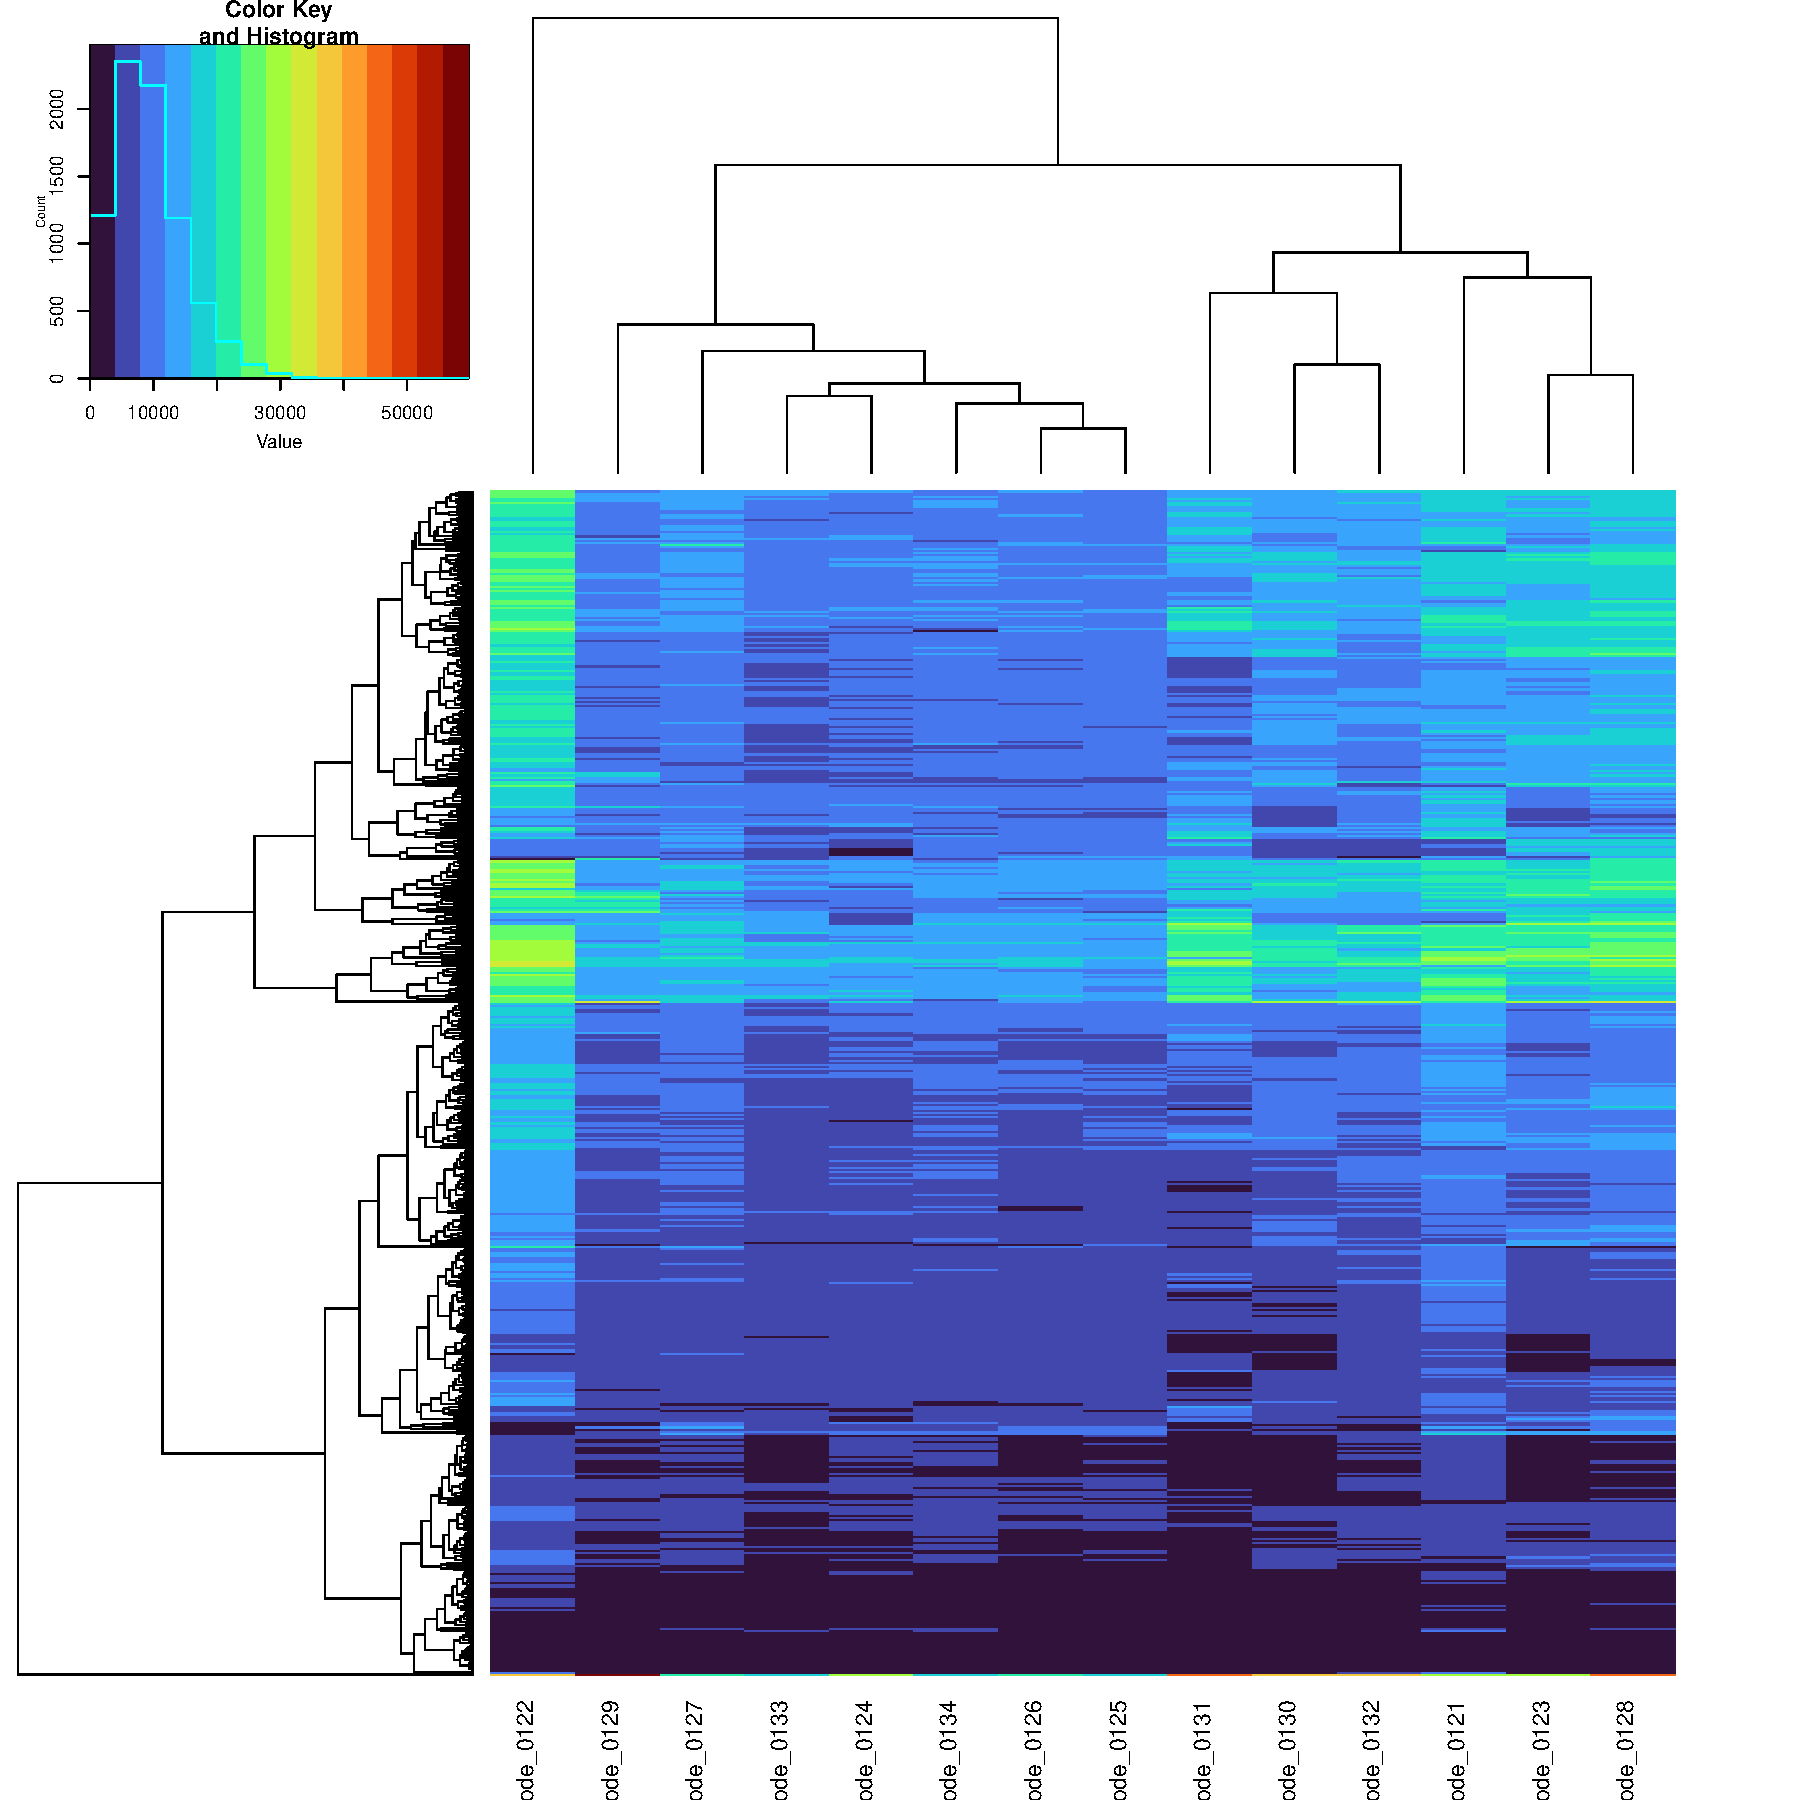
\includegraphics{C:\Users\jonat\Desktop\ngs_app_galenvs\server\records\experiment_data_140723_1449_the one\report_files/figure-latex/coverageHeatmap-1} \caption[Coverage Heatmap]{Heatmap showing the distribution of the coverage of each amplicon. Rows represent amplicons and columns represent samples}(\#fig:coverageHeatmap)
\end{figure}

\hypertarget{intersect-between-regions-covered-500x-in-at-least-half-of-the-samples}{%
\subsection{Intersect Between Regions covered \textless500X in at least Half of the Samples}\label{intersect-between-regions-covered-500x-in-at-least-half-of-the-samples}}

The following amplicons were covered less than 500X in at least half of the samples.

\begin{Shaded}
\begin{Highlighting}[]
\NormalTok{\#\# $Target}
\NormalTok{\#\# [1] "AMPL3925990" "AMPL3926201" "AMPL3091682" "AMPL2649381" "AMPL3925991"}
\NormalTok{\#\# [6] "AMPL3926093" "AMPL3926466" "AMPL3926426" "AMPL3926510"}
\end{Highlighting}
\end{Shaded}

\newpage

\hypertarget{uniformity}{%
\section{Uniformity}\label{uniformity}}

The uniformity results for each sample are shown in \textbf{\emph{table @ref(tab:uniformityTable)}}.

\begin{longtable}[t]{llll}
\caption{(\#tab:uniformityTable)Uniformity Results.}\\
\toprule
Barcode ID & Sample Name & Uniformity & Uniformity QC Check\\
\midrule
IonCode\_0121 & Sample 1 & 93.57\% & ACCEPTABLE\\
IonCode\_0122 & Sample 2 & 93.14\% & ACCEPTABLE\\
IonCode\_0123 & Sample 3 & 91.87\% & FAIL\\
IonCode\_0124 & Sample 4 & 94.17\% & ACCEPTABLE\\
IonCode\_0125 & Sample 5 & 94.25\% & ACCEPTABLE\\
\addlinespace
IonCode\_0126 & Sample 6 & 93.69\% & ACCEPTABLE\\
IonCode\_0127 & Sample 7 & 95.28\% & ACCEPTABLE\\
IonCode\_0128 & Sample 8 & 92.74\% & FAIL\\
IonCode\_0129 & Sample 9 & 94.45\% & ACCEPTABLE\\
IonCode\_0130 & Sample 10 & 91.83\% & FAIL\\
\addlinespace
IonCode\_0131 & Sample 11 & 86.14\% & FAIL\\
IonCode\_0132 & Sample 12 & 93.63\% & ACCEPTABLE\\
IonCode\_0133 & Sample 13 & 94.20\% & ACCEPTABLE\\
IonCode\_0134 & Sample 14 & 94.26\% & ACCEPTABLE\\
\bottomrule
\end{longtable}

\end{document}
